%%
%% JSAI2026 Content - v3: geDIG v2 with SP improvement and intervention experiments
%% Changes from v2:
%%   - Improved SP definition: anchor-based (CLS) path concentration
%%   - Added entropy_sign parameter for phase adaptation
%%   - Replaced F-regularization with Positive/Negative intervention experiments
%%   - Simplified layer-wise analysis (kept as supporting evidence)
%%

\title{
\jtitle{動的知識グラフの探索・統合を制御する統一ゲージの提案\\---\textit{Gauge what Knowledge Graph needs.}---}
\etitle{A Unified Gauge for Controlling Exploration and Integration in Dynamic Knowledge Graphs\\--- \textit{Gauge what Knowledge Graph needs.} ---}
}

\jaddress{{\small miyauchikazuyoshi@gmail.com}}

\author{%
\jname{宮内 和義\first}
\ename{Kazuyoshi Miyauchi}
}

\affiliate{
\jname{\first{}独立研究者}
\ename{Independent Researcher}
}

\begin{abstract}
Dynamic knowledge graphs face a fundamental ``When'' problem: when to accept new information as structure, and when to continue exploration. We propose \textbf{geDIG}, a unified gauge that quantifies this trade-off as $\F = \gednorm - \lambda(s \cdot \Delta H_{\mathrm{norm}} + \gamma \Delta \mathrm{SP})$. In this work, we improve geDIG for Transformers by (1) redefining \textbf{Shortcut Purity (SP)} as path concentration to anchor tokens (CLS), solving the dilution problem in all-pairs reachability, and (2) introducing \textbf{entropy\_sign} ($s$) to adapt the interpretation based on learning phase. We validate geDIG on two instantiations: (1) \textbf{Spatial KG (Maze)}: An agent achieves 98\% success rate while rejecting 98\% of candidate edges. (2) \textbf{Semantic KG (Transformer)}: Intervention experiments show that Positive intervention (promoting $\F \downarrow$) outperforms Negative intervention by 4.6\% accuracy, demonstrating that geDIG $\F$ is a valid learning signal. These results suggest geDIG as a general-purpose gauge for controlling exploration and integration across domains.
\end{abstract}

\begin{document}
\begingroup
\setlength{\tabcolsep}{0pt}
\maketitle
\endgroup

%% ===========================================
\section{はじめに}
%% ===========================================

動的知識グラフ（Dynamic Knowledge Graph）において，新しい情報を「いつ」構造として受け入れ，「いつ」探索を続けるべきか——この\textbf{When問題}は未解決の基本課題である．
本研究では，自由エネルギー原理（FEP）\cite{friston2010}と最小記述長（MDL）\cite{grunwald2007}を操作的に橋渡しする統一評価関数 \textbf{geDIG} (graph edit Distance and Information Gain) を提案し，この問題に原理的な解を与える．

geDIGの核心的仮説は，「\textbf{構造コストと情報利得のトレードオフ}を単一スカラーで評価すれば，知識グラフの種類によらず，探索と統合を統一的に制御できる」というものである．
本稿では，geDIGを迷路とTransformerで検証する．特に，Transformer適用における課題を解決する2つの改良を提案する：
\begin{enumerate}
    \item \textbf{SP定義の改善}：全ペア到達性からアンカー（CLS）への経路集中度へ
    \item \textbf{entropy\_sign導入}：学習フェーズに応じた解釈の切替
\end{enumerate}

%% ===========================================
\section{geDIG：統一評価関数の定義}
%% ===========================================

geDIGは，「構造を変えるコスト」と「それによって得られる情報の質」の収支を単一スカラー $\F$ で評価する．

\begin{equation}
\F = \gednorm - \lambda \left( s \cdot \Delta H_{\mathrm{norm}} + \gamma \cdot \Delta \mathrm{SP} \right)
\label{eq:gedig}
\end{equation}

各項の意味は：
\begin{itemize}
\item $\gednorm$：構造変更コスト（グラフ編集距離の正規化値）
\item $\Delta H_{\mathrm{norm}}$：エントロピー変化（選択肢の多様性）
\item $\Delta \mathrm{SP}$：経路効率の変化（ショートカット形成）
\item $s$：entropy\_sign．学習フェーズに応じて$\pm 1$を取る（後述）
\end{itemize}
具体的な計算方法はドメインごとに異なり，各実験セクションで定義する．

\subsection{entropy\_sign ($s$) パラメータ}
迷路とTransformerでは初期状態が異なる：
\begin{itemize}
    \item \textbf{迷路}：空グラフから開始し，エントロピーを獲得していく（$H: 0 \to$ 増加）
    \item \textbf{Transformer（事前学習済み）}：既に構造化された状態から開始し，タスク特化のため集中化する（$H:$ 中 $\to$ 減少）
\end{itemize}
この違いに対応するため，$s$（entropy\_sign）を導入する：
\begin{itemize}
    \item $s = +1$（基本）：エントロピー増加（延伸）が利得
    \item $s = -1$（Fine-tuning）：エントロピー減少（集中）が利得
\end{itemize}

\subsection{AG/DG 二段ゲート制御}
この $\F$ を用いて，エージェントは以下の2つのゲートを制御する．
\begin{enumerate}
\item \textbf{AG (Attention Gate)}: 0-hop評価．$g_0 > \theta_{\mathrm{AG}}$ のとき探索を起動．
\item \textbf{DG (Decision Gate)}: Multi-hop評価．$g_{\min} < \theta_{\mathrm{DG}}$ のとき統合を実行．
\end{enumerate}

\begin{figure}[t]
\centering

\includegraphics[width=0.6\columnwidth]{figs/agdg_flow.pdf}
\caption{AG/DG制御フロー．AGは局所的異常（高$\F$）を，DGは大域的効率化（低$\F$）を検知する．}
\label{fig:agdg_flow}
\end{figure}

%% ===========================================
\section{検証I：空間的KGとしての迷路探索}
%% ===========================================

\paragraph{KGとしての定式化}
部分観測迷路におけるエージェントの認知地図は，動的知識グラフの一形態である．
ノードは訪問した位置，エッジは移動可能な接続を表す．

\paragraph{geDIG成分の定義（迷路）}
\begin{itemize}
\item $\gednorm$：エッジ追加数 / 正規化定数．新しいエッジを追加するコスト．
\item $\Delta H$：\textbf{候補集合の類似度分布のエントロピー}．各候補（次の行動先）に対する類似度を確率分布とし，シャノンエントロピーを計算．$\Delta H > 0$は選択肢の多様性増加を表す．
\item $\Delta \mathrm{SP}$：\textbf{平均最短経路長の相対短縮率}．$\Delta \mathrm{SP} = (L_{\mathrm{before}} - L_{\mathrm{after}}) / L_{\mathrm{before}}$．エッジ追加によりショートカットが形成されると$\Delta \mathrm{SP} > 0$となる．
\end{itemize}

\paragraph{仮説}
geDIGのAG/DGゲートにより，高い成功率を維持しつつ，候補エッジの大半を棄却する効率的な記憶構築が可能である．

\paragraph{実験設定}
15$\times$15および25$\times$25の迷路を用いた．
パラメータは $\lambda=1.0, \gamma=1.0, \theta_{\mathrm{AG}}=0.4, \theta_{\mathrm{DG}}=0.0$．
比較対象は Random Walk と Greedy DFS．

\subsection{結果：探索と統合の自律制御}

\begin{table}[t]
\centering
\caption{迷路ナビゲーション結果}
\label{tab:maze_results}
\small
\begin{tabular}{lccc}
\toprule
手法 & 成功率 & 平均ステップ & 圧縮率 \\
\midrule
\multicolumn{4}{l}{\textbf{15$\times$15} ($n=100$)} \\
Random Walk & $0.75 \pm 0.08$ & $105.8 \pm 63.9$ & -- \\
Greedy DFS & $0.99 \pm 0.03$ & $82.1 \pm 30.8$ & -- \\
\textbf{geDIG} & $\mathbf{0.98 \pm 0.03}$ & $89.6 \pm 44.8$ & \textbf{98\%} \\
\midrule
\multicolumn{4}{l}{\textbf{25$\times$25} ($n=60$)} \\
Random Walk & $0.40 \pm 0.12$ & $242.2 \pm 143.7$ & -- \\
\textbf{geDIG} & $0.75 \pm 0.11$ & $254.1 \pm 125.4$ & \textbf{99\%} \\
\bottomrule
\end{tabular}
\end{table}

geDIGエージェントは，Random Walkを有意に上回り（McNemar検定，$p < 10^{-5}$），候補エッジの98\%を棄却しながら高い成功率を達成した（表\ref{tab:maze_results}）．

\begin{figure}[t]
\centering
\begin{minipage}{0.48\columnwidth}
  \centering
  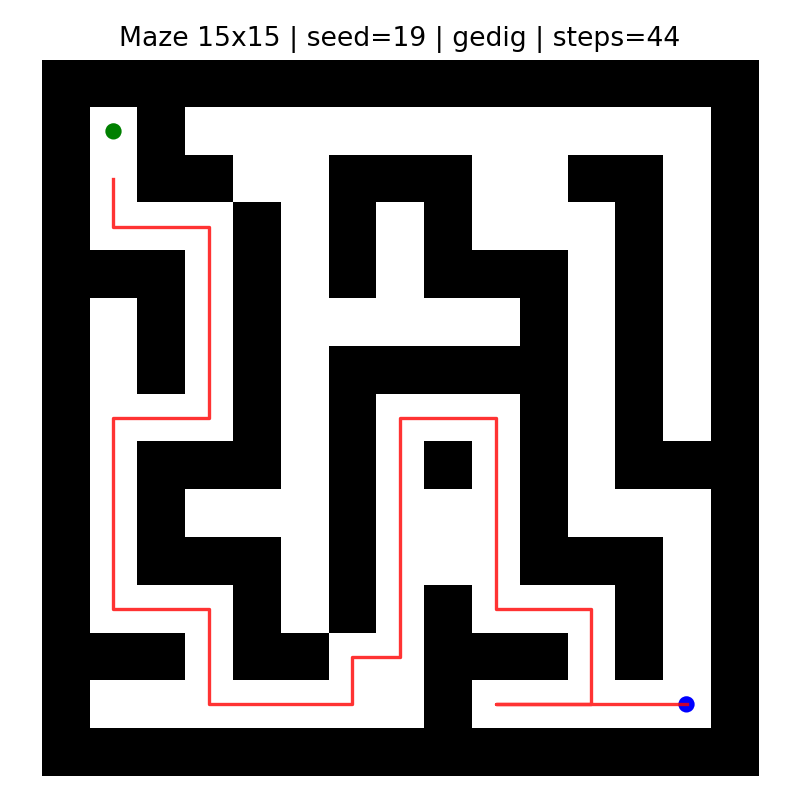
\includegraphics[width=\linewidth]{figs/maze_view.png}
  \centerline{(a) 実空間の探索軌跡}
\end{minipage}
\begin{minipage}{0.48\columnwidth}
  \centering
  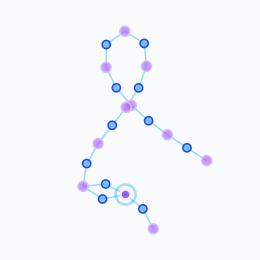
\includegraphics[width=0.9\linewidth]{figs/maze_graph_abstract.png}
  \centerline{(b) 抽象化された内部表現}
\end{minipage}
\caption{迷路探索における実空間と内部表現の対応．直線通路は圧縮され，分岐点のみが保持される．}
\label{fig:maze_process}
\end{figure}

%% ===========================================
\section{検証II：意味的KGとしてのTransformer}
%% ===========================================

\paragraph{KGとしての定式化}
TransformerのAttention行列$A_{ij}$は，トークン間の「関係の強さ」を表す．
これを閾値処理してグラフ化すると，意味的KGが得られる．

\paragraph{geDIG成分の定義（Transformer）}
\begin{itemize}
\item $\gednorm$：Attention重みの有意な変化量．閾値以上の変化をカウント．
\item $\Delta H$：\textbf{Attention分布のエントロピー}．各クエリトークンのattention分布からシャノンエントロピーを計算．$\Delta H < 0$は特定トークンへの集中を表す．
\item $\Delta \mathrm{SP}$：\textbf{CLSへの経路集中度}（下記で詳述）．
\end{itemize}

\subsection{SP（Shortcut Purity）の再定義}

従来のSP定義（全ペア到達性）は，Transformerでは意味が希釈される問題があった．
本研究では，\textbf{アンカートークン（CLS）への経路集中度}としてSPを再定義する：
\begin{equation}
\mathrm{SP} = \frac{\sum_{\mathrm{top\text{-}k}} A_{i \to \mathrm{CLS}}}{\sum_{\mathrm{all}} A_{i \to \mathrm{CLS}}}
\end{equation}
ここで，上位$k$\%の経路が全体に占める割合を測定する．
高いSP値は「少数の強い経路」（効率的なショートカット）を，低いSP値は「多数の弱い経路」（ノイズ）を表す．

\paragraph{迷路との対応}
両ドメインでSPは「効率的な経路形成」を測定する：
\begin{itemize}
    \item 迷路：平均最短経路長の短縮（ショートカット発見）
    \item Transformer：CLSへの情報集約の効率化
\end{itemize}

\subsection{実験設定}

\paragraph{モデル・タスク}
DistilBERT，SST-2感情分類．訓練2000サンプル，評価500サンプル．

\paragraph{介入方法}
geDIG $\F$に基づく正則化を適用：
\begin{itemize}
    \item \textbf{Positive介入}：$\F \downarrow$方向（SP$\uparrow$を促進）
    \item \textbf{Negative介入}：$\F \uparrow$方向（SP$\downarrow$を促進）
    \item \textbf{Baseline}：正則化なし
\end{itemize}
entropy\_sign $s = -1$（Fine-tuning用），$\alpha = 0.1$，2エポック．

\subsection{結果：geDIG Fが学習方向を予測}

\begin{table}[t]
\centering
\caption{介入実験結果（SST-2, DistilBERT, $s=-1$）}
\label{tab:intervention}
\small
\begin{tabular}{lccc}
\toprule
条件 & 精度 & mean\_F & mean\_SP \\
\midrule
Baseline & 86.8\% & 2.13 & 0.80 \\
\textbf{Positive} & \textbf{85.6\%} & 1.77 & \textbf{0.99} \\
Negative & 81.0\% & 0.63 & 0.71 \\
\bottomrule
\multicolumn{4}{l}{\scriptsize Positive $>$ Negative: 4.6\%差} \\
\end{tabular}
\end{table}

表\ref{tab:intervention}に示すように，\textbf{Positive介入がNegative介入を4.6\%上回った}．
これは，geDIG $\F$が有効な学習シグナルであることを因果的に示している．

\paragraph{SP変化の観察}
Positive介入ではSPが0.80$\to$0.99に増加（CLSへの経路集中），Negative介入では0.80$\to$0.71に減少した．
これは，SP定義がTransformerの学習ダイナミクスを正しく捉えていることを示す．

\subsection{観測：層別の構造相転移}

図\ref{fig:layer_f}にBERTの層別geDIG F値の分布を示す．
geDIG v2（SP=CLSへの経路集中度）で分析した結果：
\begin{itemize}
    \item \textbf{浅層}（0-2）：分散が大きく中央値は約7．多様な注意パターンが混在．
    \item \textbf{深層}（5-11）：中央値が約9に上昇し，外れ値（低F）が出現．構造化が進む一方，一部サンプルで効率的な経路が形成される．
\end{itemize}
この結果は，Transformerが層方向に「探索$\to$構造化」の相転移を行っていることを示唆する．

\begin{figure}[t]
\centering
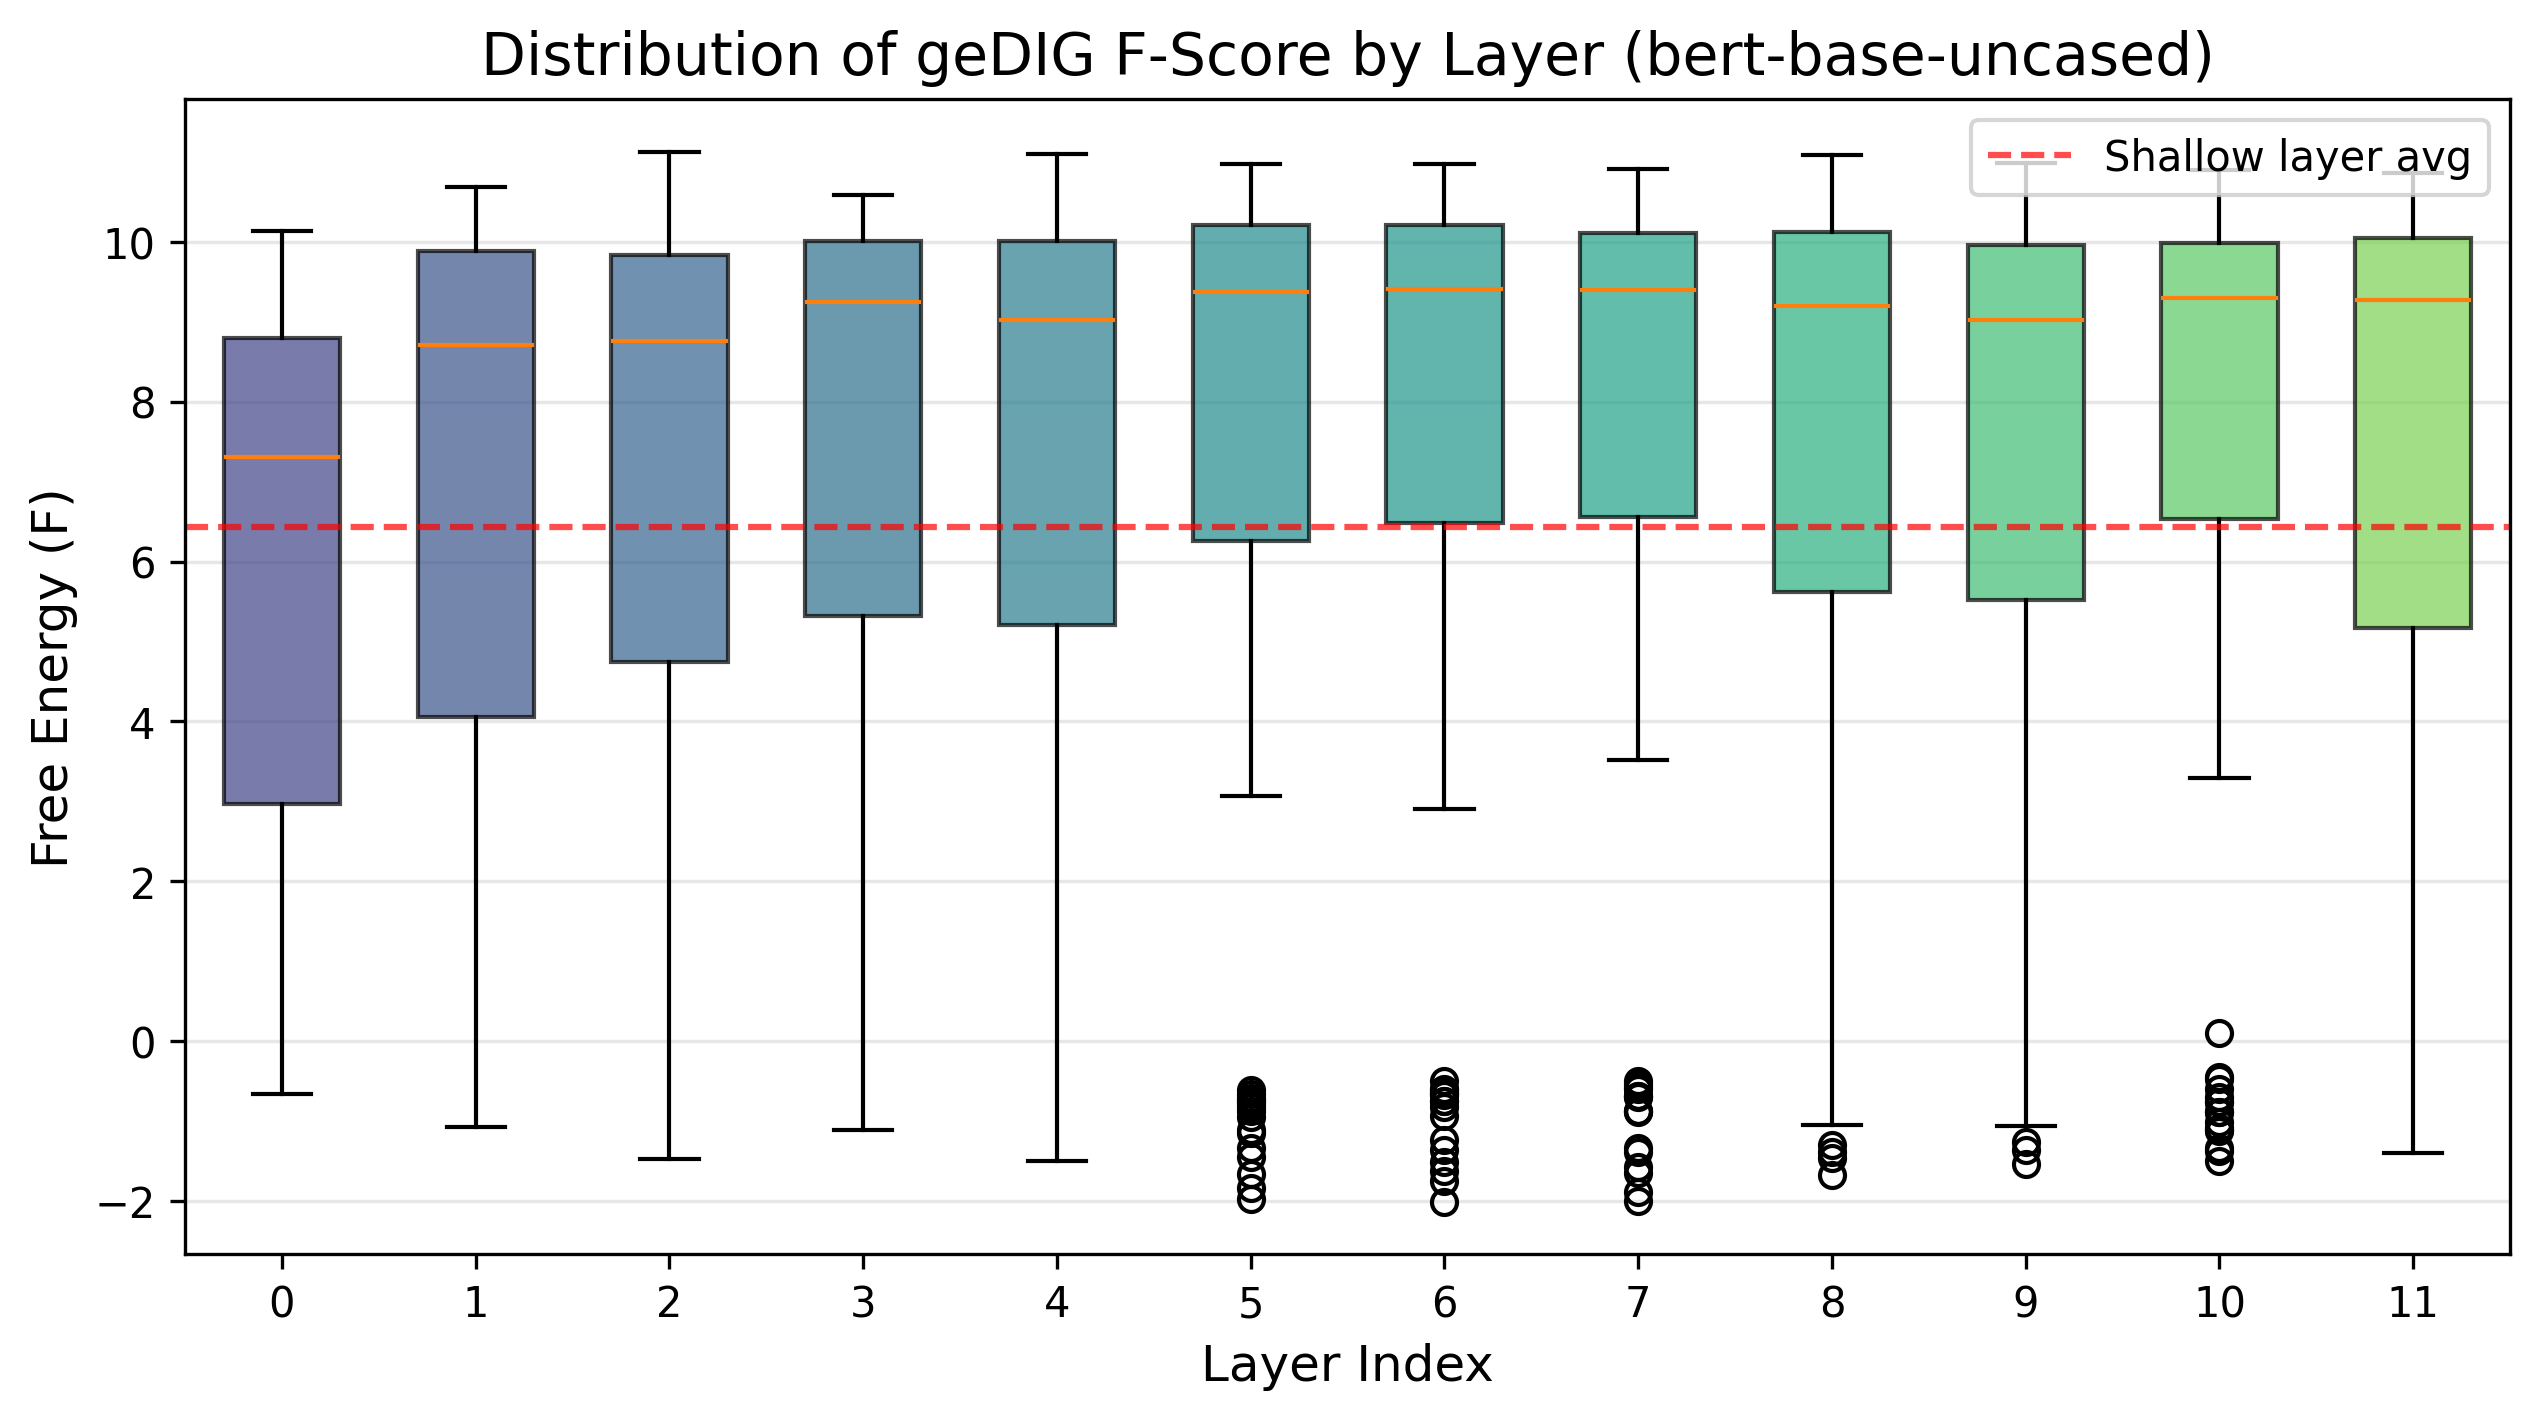
\includegraphics[width=0.85\columnwidth]{figs/layer_wise_f_v2.png}
\caption{BERTにおける層別geDIG F値の分布（geDIG v2, $s=-1$, $n=100$）．浅層で分散が大きく中央値が低い一方，深層では中央値が上昇し外れ値（低F）が出現する．}
\label{fig:layer_f}
\end{figure}

%% ===========================================
\section{考察とおわりに}
%% ===========================================

本研究では，2種類の動的KG——空間的KG（迷路）と意味的KG（Attention）——において，geDIG評価関数 $\F$ が共通の「構造化原理」として機能することを示した．

\paragraph{v2からの主な改良}
\begin{enumerate}
    \item \textbf{SP定義}：全ペア到達性$\to$アンカーへの経路集中度
    \item \textbf{entropy\_sign}：学習フェーズに応じた解釈の切替
    \item \textbf{介入実験}：Positive$>$Negativeで因果関係を実証
\end{enumerate}

\paragraph{迷路とTransformerの対応}
両ドメインに共通するのは，「構造とエントロピーのトレードオフで最適な経路効率に収束する」というプロセスである．
迷路ではゴールへのショートカット形成，TransformerではCLSへの情報集約として現れる．

\paragraph{構造生成としての学習}
従来のニューラルネットワーク学習は「重みの最適化」として定式化されてきた．
一方，geDIGの視点では，学習は「グラフ構造の生成」として捉え直せる．
重み更新の結果としてAttentionパターンが変化し，それがKGのエッジ追加・削除に対応する．
この視点は，学習を「与えられた損失関数の最小化」から「内部構造の自律的組織化」へと再解釈する可能性を示唆する．

\paragraph{内発報酬としてのgeDIG}
geDIG $\F$は外部の正解ラベルを必要とせず，ネットワーク内部の状態のみから計算できる．
これは，$\F$が\textbf{内発報酬}（intrinsic reward）として機能しうることを意味する．
迷路実験では，ゴール到達という外部報酬なしに，$\F$の最小化のみでナビゲーションが成立した．
この性質は，自己教師あり学習や継続学習への応用可能性を示唆する．

\paragraph{限界と今後の展望}
本研究は事前学習済みモデルのFine-tuningのみを検証した．
今後は，Pythia\cite{biderman2023}のチェックポイントを用いて，ランダム初期化からの学習過程全体（$H: \mathrm{max} \to \mathrm{optimal}$）を観察し，geDIGの適用範囲を拡大する予定である．

%% ===========================================
%% 参考文献
%% ===========================================
\begin{thebibliography}{99}
\bibitem{friston2010} Friston, K.: The free-energy principle: a unified brain theory?, Nat. Rev. Neurosci., 11, 127--138 (2010).
\bibitem{grunwald2007} Gr\"{u}nwald, P.~D.: The Minimum Description Length Principle, MIT Press (2007).
\bibitem{vaswani2017} Vaswani, A., et al.: Attention Is All You Need, NeurIPS (2017).
\bibitem{okeefe1978} O'Keefe, J., Nadel, L.: The Hippocampus as a Cognitive Map, Oxford University Press (1978).
\bibitem{devlin2019} Devlin, J., et al.: BERT: Pre-training of Deep Bidirectional Transformers for Language Understanding, NAACL (2019).
\bibitem{bunke1997} Bunke, H.: On a relation between graph edit distance and maximum common subgraph, Pattern Recognition Letters, 18(8), 689--694 (1997).
\bibitem{biderman2023} Biderman, S., et al.: Pythia: A Suite for Analyzing Large Language Models Across Training and Scaling, ICML (2023).

\end{thebibliography}

\end{document}
